\documentclass[]{article}

% Imports the catppuccin theme, using the mocha flavor,
% from the directory above. Actual implementation
% wouldn't need the import package unless the theme
% and the document are in different directories.
\usepackage{import}
\usepackage{xcolor}
% \usepackage{fancyhdr}
\usepackage{cancel}
\usepackage{mathtools}

% For permutations and combinations
\newcommand\Myperm[2][^n]{\prescript{#1\mkern-2.5mu}{}P_{#2}}
\newcommand\Mycomb[2]{\prescript{#1\mkern-0.5mu}{}C_{#2}}

% Colors
\definecolor{yorhabg}{HTML}{FFFFFF}
\definecolor{yorhafg}{HTML}{000000}
\definecolor{yorhagrid}{HTML}{B5AF9C}
\definecolor{mred}{HTML}{D67069}
\definecolor{mblue}{HTML}{6887A1}

\pagecolor{yorhabg}
\color{yorhafg}

\usepackage{preamble}

% Removes padding above title
\usepackage{titling}
\setlength{\droptitle}{-10em}

% Font package
\usepackage[T1]{fontenc}

\usepackage{fouriernc}

\usepackage{sectsty}
\usepackage{graphicx}
\usepackage{amsmath}
\usepackage{amsfonts}
\usepackage{amssymb}
\usepackage[skins, most]{tcolorbox}
\usepackage{enumitem}

\DeclareMathOperator{\sgn}{sgn}

\usepackage{tikz}
\usepackage{eso-pic}
\usetikzlibrary{calc,shadows.blur}
\usetikzlibrary{angles, quotes}
\usetikzlibrary{3d}

% Margins
\topmargin=0in
\evensidemargin=0in
\oddsidemargin=0in
\textwidth=6.5in
\textheight=9.0in
\headsep=0.25in

\AtBeginEnvironment{tcolorbox}{\small}

\newtcolorbox{imp}{enhanced,arc=0mm,colback=yorhabg,colframe=mred,leftrule=10mm,coltext=yorhafg,%
overlay={\node[anchor=west,outer sep=2pt] at (frame.west) {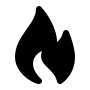
\includegraphics[width=6mm]{images/imageb.png}}; }}

\newtcolorbox{shortcut}{enhanced,arc=0mm,colback=yorhabg,colframe=mred,leftrule=10mm,coltext=yorhafg, coltitle=yorhabg, title=\texttt{Shortcut.}, 
overlay={\node[anchor=west,outer sep=2pt] at (frame.west) {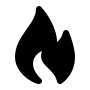
\includegraphics[width=6mm]{images/imageb.png}}; }}

\newtcolorbox{question}[1]{
    enhanced, 
    colback=yorhabg,
    colframe=mblue,
    coltext=yorhafg,
    coltitle=yorhabg,
    attach boxed title to top left={yshift*=-\tcboxedtitleheight}, 
    title=\texttt{#1},
    boxed title size=title,
    boxed title style={%
        rounded corners=northeast, 
        rounded corners=northwest, 
        colback=tcbcolframe, 
        boxrule=0pt,
    },
    underlay boxed title={%
        \path[fill=tcbcolframe] (title.south west)--(title.south east) 
            to[out=0, in=180] ([xshift=5mm]title.east)--
            (title.center-|frame.east)
            [rounded corners=5pt] |- 
            (frame.north) -| cycle; 
    },
}

\newcommand\bb[1]{\textcolor{yorhafg}{\textbf{#1}}}

\title{\textbf{CSCA67 - Assignment \#2}}
\author{Satyajit Datta \ 1012033336}
\date{\today}

\begin{document}
\maketitle

\section{Quantifiers}
For each of the following logical expressions, write a corresponding (English) mathematical statement, indicate
whether the statement is true or false, and provide a brief explanation. Universe of discourse is $\mathbb{R}$, the real numbers.

\begin{question}{1.1}
\[
\exists x \forall y,\; x + y = y
\]
\end{question}
\begin{enumerate}[label=(\alph*)]
    \item \textbf{English statement:} There exists a real number $x$ such that for all $y \in \mathbb{R}$, $x + y = y$.
    \item \textbf{Truth value:} True.
    \item \textbf{Explanation:} Let $x = 0$. Then $x + y = y$ for all $y$.
\end{enumerate}

\begin{question}{1.2}
\[
\forall x\forall y,\;((x \ne 0) \land (y \ne 0)) \leftrightarrow (xy \ne 0)
\]
\end{question}
\begin{enumerate}[label=(\alph*)]
    \item \textbf{English statement:} For all $x$, for all $y$, $x$ is not equal to $0$ and $y$ is not equal to $0$ if and only if $xy$ is not $0$.
    \item \textbf{Truth value:} True
    \item \textbf{Explanation:} For a product of 2 numbers to not equal 0, both numbers must not be 0.
\end{enumerate}

\begin{question}{1.3}
\[
\forall x\exists y,\; x^2 = y
\]
\end{question}
\begin{enumerate}[label=(\alph*)]
    \item \textbf{English statement:} For all $x$, there exists $y$ such that $x^2 = y$
    \item \textbf{Truth value:} True
    \item \textbf{Explanation:} Every real number has a square
\end{enumerate}

\begin{question}{1.4}
\[
\exists x\forall y,\; xy = 0
\]
\end{question}
\begin{enumerate}[label=(\alph*)]
    \item \textbf{English statement:} There exists an $x$ such that for all $y$, $xy=0$.
    \item \textbf{Truth value:} True
    \item \textbf{Explanation:} If $x=0$, then $xy$ is always $0$.
\end{enumerate}

\begin{question}{1.5}
\[
\exists x \exists y,\; x + y\ne y +x
\]
\end{question}
\begin{enumerate}[label=(\alph*)]
    \item \textbf{English statement:} There exists $x$, and there exists a $y$ such that x + y is not equal to y + x
    \item \textbf{Truth value:} False
    \item \textbf{Explanation:} Due to the commutative law of algebra, x + y is always equal to y + x
\end{enumerate}

\begin{question}{1.6}
\[
\exists x \forall y,\; (y \ne 0) \rightarrow (xy = 1)
\]
\end{question}
\begin{enumerate}[label=(\alph*)]
    \item \textbf{English statement:} There exists an $x$, such that for every real number $y$, if $y \ne 0$, then $xy = 1$
    \item \textbf{Truth value:} False
    \item \textbf{Explanation:} There is no set value $x$ such that $xy = 1$ for every possible $y$.
\end{enumerate}

\begin{question}{1.7}
\[
\forall y \exists x,\; (y \ne 0) \rightarrow (xy = 1)
\]
\end{question}
\begin{enumerate}[label=(\alph*)]
    \item \textbf{English statement:} For every real number $y$, there exists an $x$ such that if $y \ne 0$, then $xy = 1$
    \item \textbf{Truth value:} True
    \item \textbf{Explanation:} If $x = \frac{1}{y}$, then $xy= 1$
\end{enumerate}

\begin{question}{1.8}
\[
\forall x\forall y,\; ((x \ge 0) \land (y \ge 0)) \rightarrow \exists z, 0 \le x \le z \le y
\]
\end{question}
\begin{enumerate}[label=(\alph*)]
    \item \textbf{English statement:} For all $x$, for all $y$, if $x \ge 0$ and $y \ge 0$, then there exists a number $z$ such that $z$ lies between $x$ and $y$
    \item \textbf{Truth value:} False
    \item \textbf{Explanation:} If $y < x$, then the inequality cannot hold.
\end{enumerate}

\begin{question}{1.9}
\[
\forall x\forall y, (x \ge 0) \rightarrow ((y \rightarrow 0) \rightarrow ( x + y \ge 0))
\]
\end{question}
\begin{enumerate}[label=(\alph*)]
    \item \textbf{English statement:} For all $x$, and for all $y$, if $x \ge 0$, then $y \ge 0$ means that $(x + y) > 0$ 
    \item \textbf{Truth value:} True
    \item \textbf{Explanation:} All non-negative numbers add up to a non-negative number.
\end{enumerate}

\begin{question}{1.10}
\[
\forall x\forall y,\; ((x \ge 0) \land (y \ge 0)) \leftrightarrow (xy \ge 0)
\]
\end{question}
\begin{enumerate}[label=(\alph*)]
    \item \textbf{English statement:} For all x, and for all y, $x \ge 0$ and $y \ge 0$ if and only if $xy \ge 0$
    \item \textbf{Truth value:} False
    \item \textbf{Explanation:} If both x and y are less than 0, then xy is still greater than 0.
\end{enumerate}
\section{Negation}
For each of the following sentences:
\begin{enumerate}[label=(\alph*)]
  \item Write a logical expression that represents the English sentence.
  \item Write an English sentence that is the negation of the original sentence.
  \item Negate the expression in Step 1, and use logical equivalence rules to
  demonstrate that the result is equivalent to the logical form of the English sentence in Step 2.
\end{enumerate}

$M(x)$ stands for “$x$ is a Mathematics student”, $C(x)$ stands for “$x$ is a Computer Science student”, $S(x)$ stands
for “$x$ is a Statistics student”, $T(x, y)$ stands for “student $x$ takes course $y$” (“student $x$ is in course $y$”), $D(x)$ stands
for “$x$ is a discrete mathematics class”, $P(x)$ stands for “$x$ is a programming class”, and $L(x)$ stands for “$x$ is a
Political Science class”. Universe of discourse is students and classes. 

Do not use the shortcut $\exists!x$ in any of your solutions.
\begin{question}{2.1}
Everyone in any discrete mathematics class is either a Mathematics student, a Computer Science student, or a Statistics student.
\end{question}
\begin{enumerate}[label=(\alph*)]
    \item \textbf{Logical Expression:} $\forall x, (D(x) \rightarrow \forall y, (T(y, x) \rightarrow (M(y) \lor C(y) \lor S(y))))$
    \item \textbf{English negation:} There exists a discrete math class which has a student that is not a Mathematics, CS, or Statistics student.
    \item \textbf{Negation Proof:}
    \begin{align*}
        &\neg(\forall x, (D(x) \rightarrow \forall y, (T(y, x) \rightarrow (M(y) \lor C(y) \lor S(y))))) \quad & \\
        \implies&\exists x, \neg(D(x) \rightarrow \forall y, (T(y, x) \rightarrow (M(y) \lor C(y) \lor S(y)))) \quad & \text{Quantifier Negation} \\
        \implies&\exists x, \neg(\neg D(x) \lor \forall y, (\neg T(y, x) \lor (M(y) \lor C(y) \lor S(y)))) \quad & \text{cond.} \\
        \implies&\exists x, \neg\neg D(x) \land  \neg(\forall y, (\neg T(y, x) \lor (M(y) \lor C(y) \lor S(y)))) \quad & \text{deM.} \\
        \implies&\exists x, \neg\neg D(x) \land  \exists y, \neg(\neg T(y, x) \lor (M(y) \lor C(y) \lor S(y))) \quad & \text{Quantifier Negation} \\
        \implies&\exists x, \neg\neg D(x) \land  \exists y, \neg\neg T(y, x) \land \neg(M(y) \lor C(y) \lor S(y)) \quad & \text{deM.} \\
        \implies&\exists x, D(x) \land  \exists y, (T(y, x) \land \neg(M(y) \lor C(y) \lor S(y))) \quad & \text{d.n.} \\
    \end{align*}
    \begin{center}
        As required to show. $\blacksquare$
    \end{center}
\end{enumerate}
\vspace{0.1in}
\begin{question}{2.2}
Only Computer Science students take programming classes.
\end{question}
\begin{enumerate}[label=(\alph*)]
    \item \textbf{Logical Expression:} $\forall x, (P(x) \rightarrow \forall y, (L(y, x) \rightarrow C(y)))$
    \item \textbf{English negation:} There is a programming class which has a student that is not in CS.
    \item \textbf{Negation Proof:}
    \begin{align*}
        &\neg(\forall x, (P(x) \rightarrow \forall y, (L(y, x) \rightarrow C(y))))\quad & \\
        \implies&\exists x, \neg(P(x) \rightarrow \forall y, (L(y, x) \rightarrow C(y))) \quad & \text{Quantifier Negation} \\
        \implies&\exists x, \neg(\neg P(x) \lor \forall y, (\neg L(y, x) \lor C(y))) \quad & \text{cond.} \\
        \implies&\exists x, (\neg\neg P(x) \land \neg (\forall y, (\neg L(y, x) \lor C(y)))) \quad & \text{deM.} \\
        \implies&\exists x, (\neg\neg P(x) \land \exists y, \neg(\neg L(y, x) \lor C(y))) \quad & \text{Quantifier Negation} \\
        \implies&\exists x, (\neg\neg P(x) \land \exists y, (\neg\neg L(y, x) \land \neg C(y))) \quad & \text{deM.} \\
        \implies&\exists x, P(x) \land \exists y, (L(y, x) \land \neg C(y)) \quad & \text{d.n.} \\
    \end{align*}
    \begin{center}
        As required to show. $\blacksquare$
    \end{center}
\end{enumerate}

\begin{question}{2.3}
Non-Mathematics students take no more than two discrete mathematics classes.
\end{question}
\begin{enumerate}[label=(\alph*)]
    \item \textbf{Logical Expression:}
    \item \textbf{English negation:} There exists a non-mathematics students that takes more than two discrete math classes.
    \item \textbf{Negation Proof:}
\end{enumerate}

\begin{question}{2.4}
There is at least one Statistics student who takes a discrete mathematics class, a political science class, and no
programming classes.
\end{question}
\begin{enumerate}[label=(\alph*)]
    \item \textbf{Logical Expression:} 
    \item \textbf{English negation:} 
    \item \textbf{Negation Proof:}
\end{enumerate}

\begin{question}{2.5}
At least two Computer Science students take a Political Science class.
\end{question}
\begin{enumerate}[label=(\alph*)]
    \item \textbf{Logical Expression:}
    \item \textbf{English negation:} No more than one student takes a political science class.
    \item \textbf{Negation Proof:}
\end{enumerate}

\section{Deductive Reasoning}
For each of the following arguments, either:

• prove the argument is valid by using Rules of Inference and logical equivalence laws, OR

• prove the argument is not valid by providing a world that makes the premises true and the conclusion false.


\begin{question}{3.1}
    There is a course, which all computer science and all statistics majors take. There is a course, which all
    mathematics and all statistics majors take. Alice is a computer science student, and Bob is a mathematics
    student. Therefore, they take at least one course together.
    \medbreak
Let $M(x)$ stand for “$x$ is a mathematics major student”, $C(x)$ stand for “$x$ is a computer science major student”,
$S(x)$ stand for “$x$ is a statistics major student”, $R(x)$ stand for “$x$ is a course”, and $T(x, y)$ stand for “student
$x$ takes course $y$”. Universe of discourse is students and courses.
\end{question}

\begin{question}{3.2}
    Every CMS student is either a mathematics, computer science, or statistics major. All mathematics majors must
take calculus. All statistics majors must take probability. All computer science majors must take databases.
Therefore, each CMS student takes at least one of calculus, probability, or databases.
\medbreak
Let $D(x)$ stand for “$x$ is a CMS student”, $M(x)$ stand for “$x$ is a mathematics major student”, $C(x)$ stand for
“$x$ is a computer science major student”, $S(x)$ stand for “$x$ is a statistics major student”, and $T(x, y)$ stand for
“student $x$ takes course $y$”, $c$ stand for “the calculus course”, $p$ stand for “the probability course”, and $d$ stand
for “the databases course”. Universe of discourse is students and courses.
\end{question}
    
\begin{center}
    Conclusion we want to reach:
\end{center}
\[
    \forall x, D(x) \rightarrow (T(x, d) \lor T(x, c) \lor T(x, p))
\]
\underline{\textbf{Proof}}
\begin{flalign}
    &\forall x, D(x) \rightarrow (C(x) \lor M(x) \lor S(x)) && \text{(Premise 1)} \\
    &\forall x, M(x) \rightarrow T(x, c) && \text{(Premise 2)} \\
    &\forall x, C(x) \rightarrow T(x, d)  && \text{(Premise 3)} \\
    &\forall x, S(x) \rightarrow T(x, p)  && \text{(Premise 4)} \\
    &\text{Let } a \text{ be arbitrary} \\
    &\quad D(a) \rightarrow (C(a) \lor M(a) \lor S(a)) && \text{(1, 5, U.I)} \\  
    &\quad \text{Suppose } D(a) \\
    &\quad\quad C(a) \lor M(a) \lor S(a) && \text{(6, 7, M.P)} \\ 
    &\quad\quad \text{Suppose } C(a) \\
    &\quad\quad\quad T(a, d) && \text{(3, 9, U.M.P)} \\
    &\quad\quad\quad T(a, d) \lor T(a, c) \lor T(a, p) && \text{(10, add.)} \\
    &\quad\quad C(a) \rightarrow (T(a, d) \lor T(a, c) \lor T(a, p)) && \text{(9, 11, imp.)} \\
    &\quad\quad \text{Suppose } M(a) \\
    &\quad\quad\quad T(a, c) && \text{(2, 13, U.M.P)} \\
    &\quad\quad\quad T(a, d) \lor T(a, c) \lor T(a, p) && \text{(14, add.)} \\
    &\quad\quad M(a) \rightarrow (T(a, d) \lor T(a, c) \lor T(a, p)) && \text{(13, 15, imp.)} \\
    &\quad\quad \text{Suppose } S(a) \\
    &\quad\quad\quad T(a, p) && \text{(4, 17, U.M.P)} \\
    &\quad\quad\quad T(a, d) \lor T(a, c) \lor T(a, p) && \text{(18, add.)} \\
    &\quad\quad S(a) \rightarrow (T(a, d) \lor T(a, c) \lor T(a, p)) && \text{(17, 19, imp.)} \\
    &\quad\quad (C(a) \lor M(a) \lor S(a)) \rightarrow (T(a, d) \lor T(a, c) \lor T(a, p)) && \text{(12, 16, 20, Cases)} \\
    &\quad\quad T(a, d) \lor T(a, c) \lor T(a, p) && \text{(8, 21, M.P)} \\
    &\quad D(x) \rightarrow (T(a, d) \lor T(a, c) \lor T(a, p)) && \text{7, 22, imp.} \\
    &\forall x, D(x) \rightarrow (T(x, d) \lor T(x, c) \lor T(x, p)) && \text{(5, 23, U.G)}
\end{flalign}
\begin{center}
    As required to prove. $\blacksquare$
\end{center}

\begin{question}{3.3}
    Every CMS student takes at least two mathematics courses. In every mathematics course, all students who take
it must work hard in it. Therefore, every CMS student has at least two courses, in which they work hard.
    \medbreak
Let $C(x)$ stand for “$x$ is a CMS student”, $M(x)$ stand for “$x$ is a mathematics course”, $T(x, y)$ stand for “student
$x$ takes course $y$”, and $W(x, y)$ stand for “student $x$ works hard in course $y$”. Universe of discourse is students
and courses.
\end{question}
\begin{center}
    Conclusion we want to reach:
\end{center}
\[
    \forall x, C(x) \rightarrow (\exists y\exists z (M(y) \land M(z) \land y \ne z \land W(x, y) \land W(x, z)))
\]
\underline{\textbf{Proof.}}
\begin{flalign}
    &\forall x, C(x) \rightarrow (\exists y\exists z (M(y) \land M(z) \land y \ne z \land T(x, y) \land T(x, z))) && (\text{Premise 1}) \\
    &\forall x, M(x) \rightarrow \forall y(T(x, y) \rightarrow W(x, y)) && \text{(Premise 2)} \\
    &\text{Let } a \text{ be arbitrary} \\
    &\quad C(a) \rightarrow (\exists y\exists z (M(y) \land M(z) \land y \ne z \land W(a, y) \land W(a, z))) && \text{(1, 3, U.I)} \\
    &\quad \text{Assume } C(a) \\
    &\quad\quad \exists y\exists z (M(y) \land M(z) \land y \ne z \land W(a, y) \land W(a, z)) && \text{(4, 5, M.P)} \\
    &\quad\quad M(b) \land M(c) \land b \ne c \land W(a, b) \land W(a, c) && \text{(6, E.I)} \\
    &\quad\quad M(b) && \text{(7, simp.)} \\
    &\quad\quad \forall y, (T(y, b) \rightarrow W(y, b)) && \text{(2, 8, U.M.P)} \\
    &\quad\quad T(a, b) && \text{(7, simp.)} \\
    &\quad\quad W(a, b) && \text{(9, 10, U.M.P)} \\
    &\quad\quad M(c) && \text{(7, simp.)} \\
    &\quad\quad \forall y, (T(y, c) \rightarrow W(y, c)) && \text{(2, 12, U.M.P)} \\
    &\quad\quad T(a, c) && \text{(7, simp.)} \\
    &\quad\quad W(a, c) && \text{(13, 14, U.M.P)} \\
    &\quad\quad b \ne c && \text{(7, simp.)} \\
    &\quad\quad M(b) \land M(c) \land b \ne c \land W(a, b) \land W(a, c) && \text{(8, 11, 12, 15, 16, conj.)} \\
    &\quad\quad \exists y\exists z (M(y) \land M(z) \land y \ne z \land W(a, y) \land W(a, z)) && \text{(17, E.G)} \\
    &\quad C(a) \rightarrow (\exists y\exists z (M(y) \land M(z) \land y \ne z \land W(a, y) \land W(a, z))) && \text{(5, 18, imp.)} \\
    &\forall x, C(x) \rightarrow (\exists y\exists z (M(y) \land M(z) \land y \ne z \land W(x, y) \land W(x, z))) && \text{(3, 19, U.G)}
\end{flalign}

\begin{center}
    As required to show. $\blacksquare$
\end{center}
\section{Operations on Sets}
\section{Quantifiers and Sets}
\section{Quantifiers and Logical Equivalence}


\end{document}